\subsection{Monitoring}
Das Monitoring soll dazu dienen, die Funktionstüchtigkeit des Gerätes zu überprüfen. Zudem kann damit die Ausrichtung überprüft und die Kerntemperatur des NanoPi analysiert werden. Eine blau blinkende LED auf dem NanoPi signalisiert, dass das Gerät noch mit Strom versorgt wird und somit noch eingeschaltet ist. Um noch weitere Informationen des aktuellen Gerätes zu erhalten, muss jedoch wieder eine Verbindung via Hotspot errichtet werden. Im Anschluss kann auf die Website zugegriffen und dort weitere Daten begutachtet werden. Die Ausrichtung des Gerätes kann überprüft werden, indem der Knopf "'Stream starten"' betätigt wird. Zu diesem Zeitpunkt wird die Videoaufnahme unterbrochen und das aktuelle Video beendet. Die Verantwortung der Kamera geht vom Aufnahmeprogramm "'Avconv"' an das Streaming Programm "'Mjpg-Streamer"' über, wodurch der Webstream auf der Homepage erscheint. Nachdem die Ausrichtung der Kamera überprüft und, je nach Notwendigkeit, angepasst wurde, kann die Videoaufnahme wieder durch den zugehörigen Knopf gestartet werden. Ein Einblick in den Temperaturverlauf kann mithilfe des Knopfs "'Temperaturverlauf anzeigen"' erreicht werden. Da die Kerntemperatur einmal pro Minute ausgelesen und in ein File geschrieben wird, kann dies in einem Diagramm jederzeit begutachtet werden. Auf dem untenstehenden Bild (\fref{bTemperature}) ist ein Beispiel eines solchen Verlaufs, wie er auf der Webseite angezeigt wird. Diese Daten stammen von einem NanoPi, welcher während den Testaufnahmen in Satteins eingesetzt wurde.

\begin{figure}[H]
  \centering
  \fbox{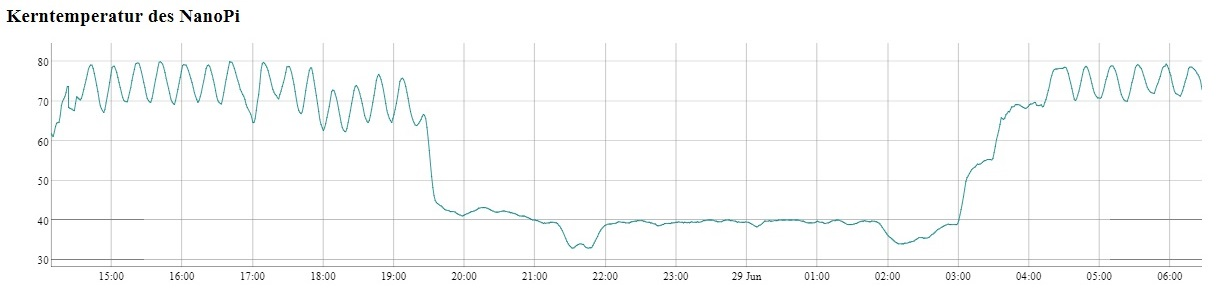
\includegraphics[width=0.99\textwidth]{Bedienungsanleitung/Temperature.jpg}}
  \caption{Temperaturverlauf eines NanoPi}
  \label{bTemperature}
\end{figure} 